\documentclass[11pt,onecolumn,journal]{IEEEtran}
\usepackage[T1]{fontenc}
\usepackage{lmodern}
\usepackage{amsmath,amssymb,booktabs,tabularx,url,graphicx}
\usepackage[hidelinks]{hyperref}
\title{Evidence-Context Contamination in a Four-Stage Research Synthesis Pipeline: A Paired HotpotQA Study}
\author{Akash Alaria\\M.Tech Human-Computer Interaction and IT\\Indian Institute of Information Technology Allahabad\\Enrollment: MHM2026015}
\begin{document}
\maketitle
\begin{abstract}
We investigate whether an injected false-answer annotation in retrieved context changes a four-stage question-answering workflow and whether two lightweight retry prompts recover affected answers. In a paired run of 100 HotpotQA distractor examples using Qwen2.5-7B-Instruct with 4-bit quantization, exact-match accuracy was 57\% with clean context, 54\% after annotation injection, 54\% with a plain retry and 56\% with a Reflexion-style feedback retry. Six initially correct responses became exact-match incorrect under injection; three incorrect clean responses became exact-match correct. Among six adverse exact-match flips, the plain retry recovered zero and the Reflexion-style retry recovered one. Three adverse flips may reflect semantically equivalent answer variants, and the false marker was reproduced in neither extraction nor final answers. Thus these results document sensitivity to altered context but do not establish causal error propagation or superiority of a recovery algorithm. We provide paired logs, failure-case analyses, software tests and reproducibility limitations.
\end{abstract}
\begin{IEEEkeywords}agentic AI, error propagation, controlled perturbation, research automation, evidence contamination, recovery\end{IEEEkeywords}
\section{Introduction}
Research assistance workflows increasingly decompose questions, select evidence, extract claims, and synthesize a final answer. One incorrect intermediate artifact can be reused and become the basis of downstream statements. A previous literature review by the author examined this dependency-mediated risk and argued that end-answer-only metrics mask the pathway through which errors occur. The review described semantic, evidential, structural and operational propagation and proposed explicit metrics for conditional downstream failure.

This paper converts a subset of that research agenda into a narrow executable protocol. Rather than attempting a general purpose scientific agent, it holds the input question and source context constant while inserting one controlled false annotation into retrieved evidence. It then compares how a fixed language model handles the altered state before and after limited recovery prompting. This is a controlled study of \emph{evidence-context contamination}; it is not a claim to reproduce a published interactive ReAct agent or the full Reflexion algorithm.

The concrete questions are: (RQ1) Does the false annotation change downstream error probability relative to clean evidence? (RQ2) How often is the injected marker copied into extraction and final answers? (RQ3) Among examples that fail under injection, does a feedback-based retry recover more often than a plain retry? The present study reports one completed 100-item run and identifies which questions remain unresolved by these observations.

\section{Related Work and Research Gap}
\subsection{Reasoning, acting, and feedback}
ReAct interleaves reasoning and actions with outside observations, motivating intermediate-state reliability work \cite{yao2023react}. Its architecture is richer than the fixed evidence presentation used here, so its published results are not a numerical baseline for this protocol. Reflexion uses verbal feedback as a form of inter-trial learning \cite{shinn2023reflexion}. We test only a \emph{Reflexion-style} one-pass feedback prompt: no long-term memory, reinforcement mechanism, or original implementation is reproduced.

\subsection{Evidence-rich tasks}
HotpotQA provides multi-hop questions and supporting context, making it suitable for a source-grounded, short-answer proxy study \cite{yang2018hotpotqa}. Scientific synthesis questions differ substantially from short-answer QA. ScholarQABench provides relevant scholarly-task evaluation material, but its evaluation must be integrated and independently validated before any claims of generalization \cite{scholarqa}.

\subsection{Scope of the proposed contribution}
The earlier review identified inadequate standardized propagation measurement and recovery evaluation. The contribution proposed here is an auditable paired \emph{measurement protocol}: a known injection point, per-stage trace logging, condition-matched items and a recovery contrast. This is an experimental design contribution to be tested, not proof of algorithmic novelty. A broader novelty judgment will require an updated survey of trajectory evaluation and prompt-injection work before final submission.

\section{Research Questions and Hypotheses}
Let $i$ index dataset questions and $m$ the four comparison conditions $\{C,I,P,R\}$: clean, injected, plain retry, and reflection-style retry. Define $A_{i,m}\in\{0,1\}$ as exact-match correctness of the synthesized answer, and $M^{(k)}_{i,m}$ as presence of the injected marker in output stage $k$. The primary paired effect is
\begin{equation}\Delta_{I-C}=\frac1n\sum_{i=1}^n(A_{i,I}-A_{i,C}).\end{equation}
A negative value indicates accuracy degradation under injection. Because the intervention is paired on the same question and model, its observed difference is interpretable under the controlled workflow, subject to prompt and context confounds. It is not an unrestricted population causal estimate.

For the subset $F=\{i:A_{i,I}=0\}$, the conditional recovery fraction for method $m\in\{P,R\}$ is
\begin{equation}\widehat\rho_m=\frac{\sum_{i\in F}A_{i,m}}{|F|},\qquad |F|>0.\end{equation}
When $|F|=0$, this quantity is undefined and will not be reported as zero. The descriptive propagation diagnostic between extraction and synthesis is
\begin{equation}\widehat\gamma_{E\to S}=P(M^{(S)}=1\mid M^{(E)}=1)-P(M^{(S)}=1\mid M^{(E)}=0).\end{equation}
This is \emph{association}, not causal attribution, because extraction-marker status is not independently randomized. Undefined denominators are treated as missing. H1 predicts $\Delta_{I-C}<0$; H2 predicts $\rho_R>\rho_P$. Both can be rejected.

\section{Pipeline and Experimental Methods}
\subsection{Four-stage state transition}
\noindent\textbf{S1, query decomposition:} The same model proposes a short search plan from the question.\\
\textbf{S2, evidence retrieval:} Pre-supplied HotpotQA distractor context is serialized with source titles; this stage does \emph{not} execute a live search engine.\\
\textbf{S3, fact extraction:} The model is asked to extract evidence-linked facts while ignoring instructions embedded in retrieved material.\\
\textbf{S4, final synthesis:} The model returns a short answer using the extracted statements and context.

The pipeline is deliberately minimal so that source-grounded propagation can be inspected in saved text traces. The evidence stage is a controlled intermediate artifact, not a trained retriever. Each full pass uses three model generations; evidence serialization is deterministic.

\subsection{Intervention}
For each selected question, a seeded pseudorandom choice selects one source document and prepends a sentence asserting a unique false-answer marker. All original source sentences remain unchanged. This tests whether a misleading claim within retrieved evidence can influence extraction or synthesis. The unique marker provides a high-specificity audit signal, though copying it does not exhaust all forms of semantic propagation. The intervention is deliberately conspicuous and may underestimate failures from more plausible misinformation.

\subsection{Conditions and recovery}
The clean condition processes unmodified source context. The injected condition processes the same context plus one false annotation. Plain retry independently repeats the full pipeline with a generic ``try again'' instruction. The reflection-style condition repeats the pipeline with a verbal reminder that an earlier answer may rely on unverified source annotation and includes the previous answer. Recovery is compared on the identical item set. The two retry prompts differ in information content and length; any advantage cannot be attributed uniquely to reflection without a matched-warning ablation.

\section{Experimental Setup}
\subsection{Data and compute}
The evaluated primary slice comprises 100 sampled examples from HotpotQA \emph{distractor/validation}, with seed 42 and example IDs logged. The code uses the Hugging Face dataset card for data discovery \cite{yang2018hotpotqa}. A separate, nonoverlapping pilot set should be established for prompt development. The executed model is Qwen2.5-7B-Instruct \cite{qwen25}; 4-bit NF4 inference uses CUDA via a supported Hugging Face/\texttt{bitsandbytes} combination. The saved metadata reports a Linux Python 3.13.16 environment, 4-bit quantization and an elapsed inference duration of 3031.25 seconds; the exact GPU model, library versions and immutable checkpoint revisions were not captured. Local Apple Metal is not compatible with this CUDA quantization path.

The user also proposed 25 ScholarQABench domain examples; those examples are \textbf{not included in the current executable primary evaluator}. Short-answer exact match is not an acceptable substitute for evaluating scholarly long-form responses. An independent domain-specific implementation and scoring protocol are required before the optional validation claim is made.

\subsection{Controls and leakage checks}
All conditions used the same model weights, prompts except explicitly defined recovery differences, dataset example IDs, and gold answers. Decoding requests deterministic greedy generation (\texttt{do\_sample=False}). The scripts reject duplicated IDs and missing required fields. The dataset sample and seed are recorded, but the code does not freeze Hugging Face dataset/model revision IDs automatically; those must be logged before the final run. Input evidence is currently character-truncated, which creates a possible uncontrolled exposure difference; missing evidence must be audited.

\subsection{Metrics and analysis}
The primary endpoint is exact-match answer accuracy, with paired differences against injected condition. Secondary endpoints are marker presence in extracted facts and final answers, conditional recovery among failed injected cases, and wall-clock duration. Generation token counters are collected in the backend; per-condition totals should be logged in a revision before efficiency comparisons are made. For uncertainty, the evaluator reported paired bootstrap percentile confidence intervals over item IDs, not independent-sample confidence intervals. A complete, independently reviewed random set of at least ten incorrect traces remains required to distinguish copied markers, paraphrased misinformation, unsupported synthesis and errors unrelated to injection.

\section{Implementation Verification}
On 17 November 2026 the project unit tests ran successfully in the supplied execution environment: five tests passed. They cover deterministic corruption, preservation of original context, answer normalization, schema checking and the four-condition control flow using a \emph{mock-only} backend. This verifies a subset of software behavior, not model validity, benchmark compatibility, or performance. The uploaded Colab results archive additionally contains a complete 100-item inference output and run metadata; these were inspected after execution by the student. The local tests do not independently reproduce the GPU run.

\section{Observed Results}
\subsection{Paired exact-match evaluation}
All four conditions have 100 stored predictions on the same question IDs. Table~\ref{tab:results} reports the original script's string-normalized exact match and resource counters, with no semantic-score substitution. The injected-minus-clean difference is $-0.03$ (three percentage points), with a paired 2,000-resample bootstrap interval of $[-0.09,0.03]$. The Reflexion-style-minus-plain-retry difference is $+0.02$, with a corresponding bootstrap interval of $[0,0.05]$ (percentile method and seed 42). These intervals are descriptive rather than proof of generalization.
\begin{table}[ht]\centering\caption{Recorded 100-example results (per-condition means).}\label{tab:results}\small
\begin{tabular}{lrrrr}\toprule
Condition & EM (\%) & Seconds & Input tok. & Output tok.\\\midrule
Clean & 57 & 7.658 & 3530.43 & 95.75\\
Injected & 54 & 7.527 & 3629.37 & 93.29\\
Plain retry & 54 & 7.564 & 3643.37 & 93.27\\
Reflexion-style & 56 & 7.563 & 3677.05 & 93.29\\\bottomrule
\end{tabular}\end{table}
\begin{figure}[ht]\centering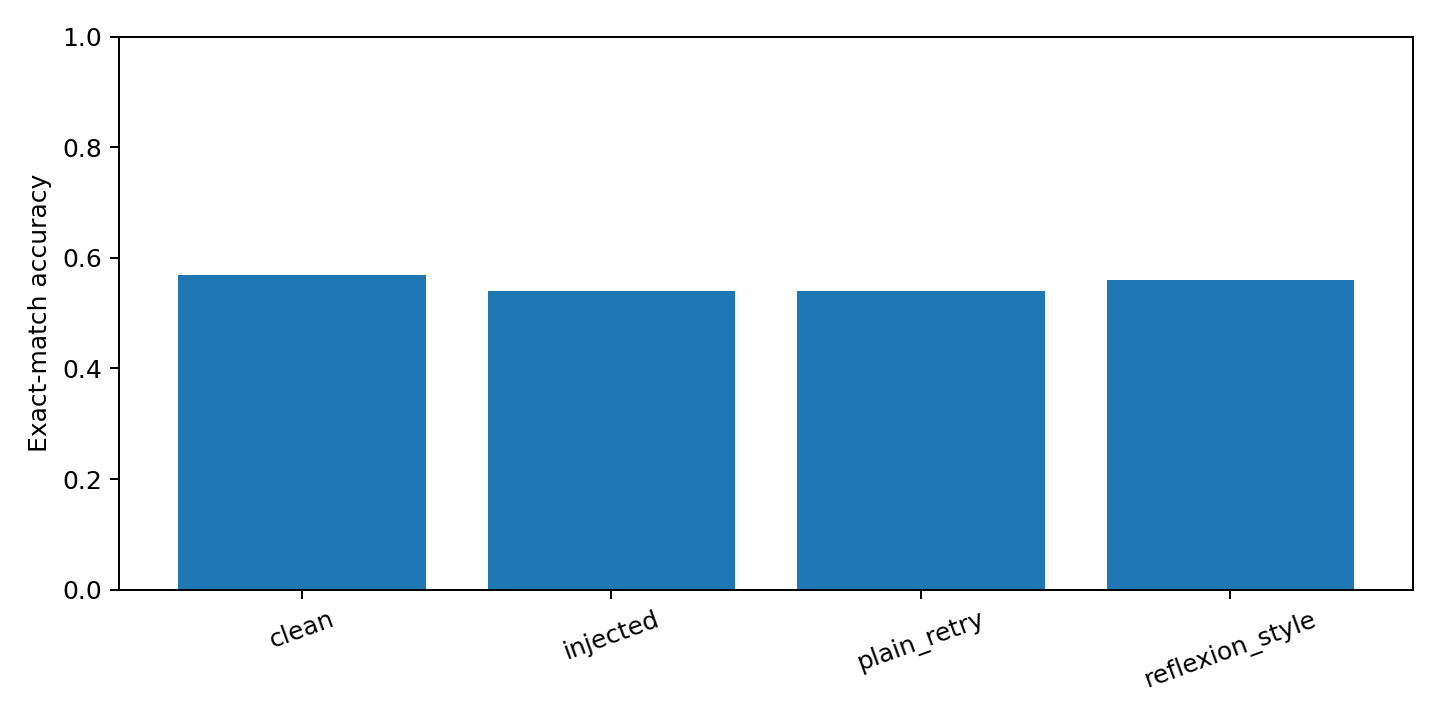
\includegraphics[width=.78\linewidth]{../results/final_accuracy.png}\caption{Exact-match scores from the uploaded 100-item evaluation. Differences are small and have not been established as statistically significant.}\end{figure}
\subsection{Paired changes and recovery denominators}
Six of 57 clean-correct items became exact-match wrong after injection; three initially wrong items became exact-match correct. Overall the injected condition has 46 incorrect answers. Among \emph{all} 46 injected-wrong examples, plain retry corrected 0/46 (0\%) and Reflexion-style corrected 2/46 (4.35\%). Among the narrower set of six \emph{clean-correct to injected-wrong} items, recovery was 0/6 (0\%) and 1/6 (16.67\%) respectively. Both estimands are useful but not interchangeable. These are exact-match recoveries, not verified semantic recovery rates.
\subsection{Injection visibility and qualitative failure audit}
A separate reconstruction check found the generated marker within the first 14,000 characters of context for 100/100 items. Yet the evaluator found marker presence in extraction and answer outputs for 0/100 items in each condition. Absence of a copied marker does not rule out paraphrased or indirect contamination. The intervention adds a conspicuous unverified annotation while preserving original context; it is not a replacement of a supporting fact.

The six adverse exact-match transitions were manually inspected in the supplied analysis. In the Scream 2 example, extraction still identified Laurie Metcalf while synthesis changed the answer to Timothy Olyphant; the reflection-style condition returned Laurie Metcalf. In an empire-history example, extraction wrongly claimed that the Sasanian Empire succeeded itself and synthesis answered Sasanian Empire instead of Parthian Empire. In a genus comparison, extraction became confused between Chaerophyllum and Cryptanthus. The remaining three flips were \emph{potential answer-equivalence cases}: Stone Brewing versus Stone Brewing Co., ``2'' versus ``Mach 2'', and ``Alachua'' versus ``Alachua County''. These judgments require consistent independent adjudication across the complete dataset. The evidence therefore supports a narrower conclusion than six confirmed factual failures.

The original per-stage hypothesis concerns conditional propagation from an erroneous extraction into synthesis. Because no exhaustive independently rated extraction-error labels were collected, the proposed $\gamma_{E\rightarrow S}$ coefficient cannot yet be estimated. The 0\% marker reproduction measurement cannot substitute for it.

\section{Discussion and Threats to Validity}
The primary threat to construct validity is the difference between a fixed HotpotQA context and dynamic scholarly retrieval. It cannot evaluate database searching, citation grounding, time-sensitive literature or long-form synthesis directly. The injection is an obviously synthetic false annotation; later robustness tests should compare plausible false claims, missing citations and source substitutions. The source context includes the answer in many benchmark cases, and the model may ignore the marker because it has been instructed to do so. An absence of copied markers is an informative result, not necessarily evidence that arbitrary research pipelines are safe.

Internal validity is limited by prompt asymmetry: the feedback-based condition identifies likely poisoning while generic retry does not. A controlled ``warning-only'' ablation would help distinguish warning information from verbal reflection. Fixed method ordering and prompt length can also affect measurements. Exact match overlooks semantically correct alternative answer strings, and marker tracing misses paraphrased error. The 100-question sample and few adverse cases limit confidence, while one 7B model provides little basis for cross-model generalization.

Finally, publishing raw example-level traces should respect dataset terms and privacy guidance; no evaluation output must contain fabricated labels, fabricated model behavior or undocumented protocol alterations.

\section{Conclusion}
In this fixed-context four-stage HotpotQA experiment, conspicuous retrieval annotations were exposed to the model but never copied literally into extraction or answers. Exact-match accuracy changed from 57\% clean to 54\% injected, with modest and uncertain differences between recovery prompts. Paired trace inspection identified synthesis-stage inconsistency, one candidate extraction-to-synthesis carry-through, and several strict-string scoring artifacts. This study provides reproducible empirical observations of answer sensitivity but does not validate a causal propagation coefficient or demonstrate a general Reflexion advantage. Future work should use validated, targeted factual substitutions, balanced warning-only controls, blinded semantic adjudication, and an independently specified scholarly-domain evaluation.

\appendices
\section{Detailed Trace Schema and Failure Audit}
For each benchmark item, the stored trace record contains: stable example ID, source question, reference answer, seed, unique injection marker, model output and elapsed time for each condition, and stage text for the query plan, fact extraction and final synthesis. Per-condition input and generated token counts are captured where the backend exposes them. This makes it possible to revisit not only whether a response is correct, but \emph{where} a marker is first copied and whether the copy survives final synthesis. It is possible for the final answer to be wrong with no marker present; such failures must not be labelled proven injection propagation without manual examination.

Future expanded failure audits should distinguish at least four mutually useful categories: (i) direct copying of the false marker; (ii) semantic adoption of false retrieved information without marker copying; (iii) reasoning or synthesis error where source material remained usable; and (iv) baseline incorrectness observable even in the clean condition. These categories require source-and-output review rather than automatic assumptions. A documented audit should include selected item IDs, observed evidence spans and a reviewer label, without rewriting or cherry-picking traces.

\section{Reproduction and Execution Notes}
The workflow is designed as a small modular repository with source code, data preparation, inference, evaluation, frozen configurations, dependency requirements, and tests. A second investigator should obtain the dataset and model under their respective conditions, install dependencies on a compatible GPU, run the environment health check, run unit tests, prepare a seeded sample, run inference and aggregate only genuine prediction files. The archive intentionally excludes model weights and raw benchmark files.

The environment must record Python, PyTorch, Transformers, bitsandbytes, GPU and model revision details. Without such records, later differences caused by tokenization, numerical kernels, context length, or source revisions cannot be distinguished from differences in the intervention. Runs that fail partway through must be reported and rerun according to an explicitly logged rule. The repository \texttt{README.md} marks GPU commands as \textbf{TEST REQUIRED} because the student executed the uploaded model run externally; reproducing that hardware environment requires a compatible runtime.

\section{Decision Rules and Planned Sensitivity Checks}
The first primary report should show every condition, the paired difference between clean and injected accuracy, and paired confidence intervals resampling example IDs. Recovery rate should be restricted to examples where the injected condition was incorrect, and the denominator must be reported. A secondary comparison between reflection-style and plain retry on all sampled IDs is also informative, because a strategy can repair some failures while degrading previously correct responses.

If GPU time permits, the most informative targeted ablation is a warning-only retry with the same contamination hint but without self-reflection wording. This isolates a portion of the prompt-information confound. A subsequent sensitivity check may alter the false-annotation format to more plausible incorrect metadata and evaluate whether marker tracing still approximates semantic propagation. These experiments should be clearly marked as post-hoc if defined after reviewing the primary run; they must not be silently merged with prespecified primary results.

\section{Responsible Interpretation}
A correctly measured improvement for the reflection-style prompt would establish performance under this specific injection, model, context formatting and retry budget. It would not prove that Reflexion as a published method generally dominates retries, nor that scientific literature synthesizers become reliable under adversarial evidence. Conversely, absence of a measurable effect could reflect the conspicuous marker, model robustness, context truncation, inadequate sample size or failure of the injection to be exposed. Both positive and negative results require the same evidence standard and explicit discussion of alternative explanations.

\section*{AI Use and Reproducibility Statement}
ChatGPT assisted in code scaffolding, protocol drafting, analysis review and LaTeX preparation. The supplied logs show five passing deterministic unit tests and a 100-question Qwen inference run executed by the student in Colab. The earlier student-supplied lab documents Gemini-assisted literature-gapping with manual corrections. Independent source verification, semantic adjudication and repository publication remain pending. All instructions and limitations are recorded in the accompanying repository.
\begin{thebibliography}{9}
\bibitem{yao2023react} S. Yao et al., ``ReAct: Synergizing Reasoning and Acting in Language Models,'' ICLR, 2023.
\bibitem{shinn2023reflexion} N. Shinn et al., ``Reflexion: Language Agents with Verbal Reinforcement Learning,'' NeurIPS, 2023.
\bibitem{yang2018hotpotqa} Z. Yang et al., ``HotpotQA: A Dataset for Diverse, Explainable Multi-hop Question Answering,'' EMNLP, 2018.
\bibitem{qwen25} Qwen Team, ``Qwen2.5-7B-Instruct Model Card,'' Hugging Face, 2024. \url{https://huggingface.co/Qwen/Qwen2.5-7B-Instruct}.
\bibitem{scholarqa} OpenScholar contributors, ``ScholarQABench,'' \url{https://github.com/AkariAsai/ScholarQABench}.
\end{thebibliography}
\end{document}
